\subsubsection{Aufgabe der Komponente}
Über den Broadcast erhält der Benutzer eine Vielzahl an Nachrichten von anderen Benutzern, von denen einen Großteil für ihn irrelevant sind. Der semantische Filter ist dafür verantwortlich, dem Benutzer nur die für ihn interessanten Nachrichten passieren und in seine Wissensbasis einfließen zu lassen. Er ist damit neben dem Broadcast die wichtigste Komponente dieser Arbeit. Neben dem bereits beschriebenen Eingangsfilter gibt es noch einen Ausgangsfilter, der für die etwaige Weiterleitung von Nachrichten an andere Peers verantwortlich ist. 
\\Die Benutzer können ihre Filter über ein Menü innerhalb des Profilbereichs einstellen, wobei dies optional ist. Wenn keine Filter gesetzt sind, werden alle Nachrichten akzeptiert und weitergeleitet, sofern diese nicht bereits zuvor empfangen worden sind. \newline
\begin{figure}[H]
	\centering
	\makebox[\linewidth][c]{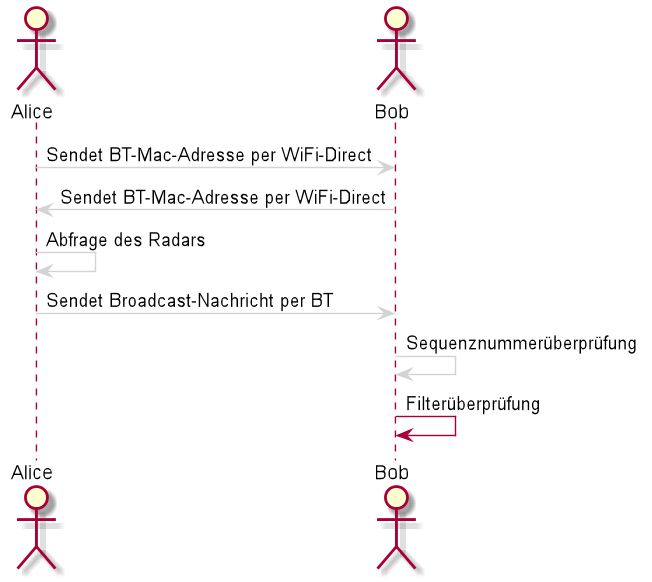
\includegraphics[width=0.6\linewidth]{semanticFilter/images/communicationComps.png}}%
	\caption{Die Broadcast-Komponente innerhalb des Nachrichtenaustauschs}
	\label{fig:filterComp}
\end{figure}
\newpage
\subsubsection{Architektur}

Der semantische Filter gliedert sich in verschiedene Teilfilter. Diese Trennung richtet sich nach den bereits bekannten Dimensionen des Shark Frameworks. Um den Gesamtfilter mit den kleineren Teilfiltern dynamisch zusammensetzen zu können, wurde das Entwurfsmuster Kompositum gewählt. Mit Hilfe dieses Musters müssen nur jeweils die Teilfilter gesetzt werden, die für den Benutzer auch eine Relevanz haben. Die folgende Klassenhierarchie verdeutlicht dieses Verhältnis:
\begin{figure}[H]
	\centering
	\makebox[\linewidth][c]{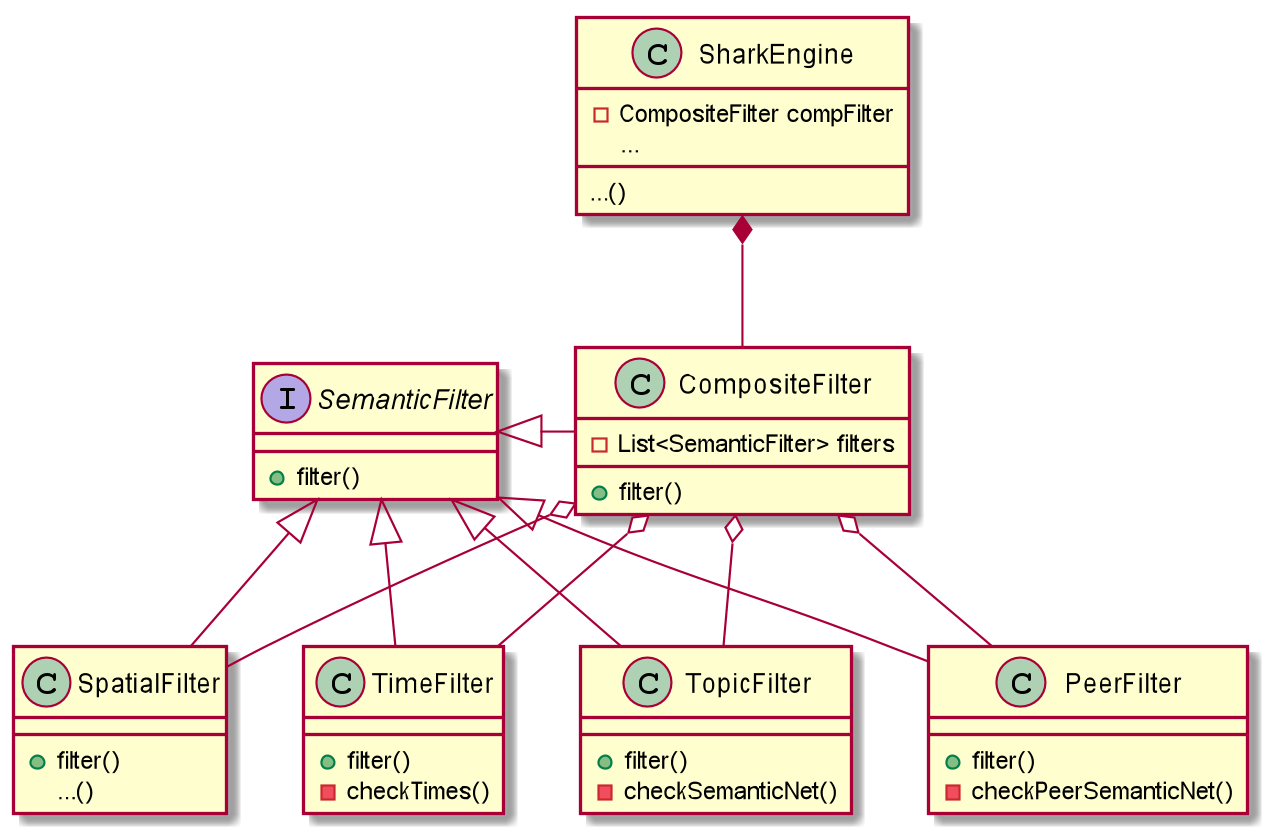
\includegraphics[width=0.8\linewidth]{semanticFilter/images/compositeFilter.png}}%
	\caption{Klassenhierarchie des semantischen Filters (Auszug)}
	\label{fig:filterStructure}
\end{figure} 
\begin{itemize}
	\item Die \textit{SharkEngine} enthält das Kompositum und stellt Methoden zur Erzeugung und Anpassung dafür bereit. Weiterhin ist diese Klasse von der App aus erreichbar, wodurch über die App abhängig von den Eingaben des Benutzers die Filter gesetzt oder entfernt werden können.
	\item Das Interface \textit{SemanticFilter} wird von allen Teilfilterklassen und der Kompositumsklasse implementiert. Die einzige zu implementierende Methode ist dabei die Filtermethode, die einen booleschen Wert zurückliefert.
	\item Der \textit{CompositeFilter} besitzt, ermöglicht durch Polymorphismus, eine Liste aus allen Teilfiltern. Bei Aufruf der Filtermethode werden sämtliche Teilfilter angewandt, die sich in der Liste befinden. Näheres dazu befindet sich im Unterkapitel 7.3.1 Code. \\
	\item Die Relevanz der Themen wird durch den \textit{TopicFilter} geprüft. Der Filter kann für die beiden Dimensionen Topics und Types verwendet werden.
	\item Die Dimensionen Sender, Approvers und Receivers werden durch den PeerFilter abgedeckt. Da die Dimension Sender im Gegensatz zu Approvers und Receivers nur ein SemanticTag, jedoch kein SemanticNet enthält, findet eine Fallunterscheidung am Anfang der Methode statt.
	\item Der \textit{TimeFilter} kontrolliert, ob sich mindestens einer der Zeiträume, die sich im semantischen Profil und in der empfangenen Nachricht befinden, überschneidet. 
	\item Die spatiale Auswertung findet im \textit{SpatialFilter} statt, sie wurde im Rahmen einer Bachelorarbeit von Maximilian Oehme entwickelt.
\end{itemize}

\subsubsection{Code}
Wie bereits im Überblick angerissen, führt der \textit{CompositeFilter} keine eigene semantische Filterung durch, sondern lässt dies fachgerecht von den Teilfiltern ausführen. Im folgenden Codeausschnitt ist erkennbar, dass der sequentielle Aufruf der Teilfilter sofort abgebrochen wird, wenn ein Teilfilter ein \textit{false} liefert.\newline
\lstset{language=Java, caption=Filtermethode im Kompositum, label=DescriptiveLabel, numbers=left, numbersep=1em, breaklines=true, basicstyle=\small}
\begin{lstlisting}
boolean isInteresing = true;
int i = 0;
while (isInteresing && i < childFilters.size()) {
isInteresing =  childFilters.get(i).filter(message, newKnowledge, entryProfile);
i++; }
return isInteresing;
\end{lstlisting}
Angenommen es handelt sich bei der ersten Iteration der Schleife um eine Instanz der Klasse \textit{TopicFilter}, welche ihre Filtermethode aufruft, dann würde es zunächst zur folgenden Auswertung kommen:\newpage
\lstset{language=Java, caption=Filtermethode des TopicType Filters (Auszug), label=DescriptiveLabel, numbers=left, numbersep=1em, breaklines=true, basicstyle=\small}
\begin{lstlisting}
if (activeEntryProfile == null) return true;
switch (dimension){
  case TOPIC:
    if (activeEntryProfile.getTopics() instanceof SemanticNet) {
	  isInteresting = checkSemanticNet(activeEntryProfile.getTopics(), newKnowledge);
	}
	else {
	  isInteresting = checkSemanticTag(newKnowledge, activeEntryProfile);
    }
break;
\end{lstlisting}
Es wird zunächst, wie auch bei allen anderen Teilfiltern, überprüft, ob überhaupt ein semantisches Profil vom Benutzer gesetzt worden ist. Falls nicht, wird die Auswertung sofort mit einem \textit{true} als Rückgabewert beendet. Anschließend wird wie auch beim \textit{PeerFilter} die Dimension bestimmt, welche vom Filter ausgewertet wird. In Zeile vier von Listing 11 wird überprüft, ob es sich nur um ein einzelnes Tag oder um ein gesamtes SemanticNet handelt. Dadurch wird der Besonderheit in Shark Rechnung getragen, dass eine Dimension entweder durch ein einzelnes Tag oder durch ein komplettes semantisches Netz beschrieben werden kann. Der folgende Auszug zeigt die Auswertung eines semantischen Netzes:\newline
\lstset{language=Java, caption=Auswertung des semantischen Netzes (Auszug), label=DescriptiveLabel, numbers=left, numbersep=1em, breaklines=true, basicstyle=\small}
\begin{lstlisting}
SemanticNet resultNet = SharkCSAlgebra.contextualize(inputNet, profileSet, fp);
	if (resultNet == null || resultNet.isEmpty()) {
		return false;
	}
	else {
		return true;
	}
\end{lstlisting}\newpage
Für die Auswertung wird die vom SharkFramework bereitgestellte Funktionalität der Kontextualisierung von semantischen Netzen benutzt. Bei der Kontextualisierung soll das gemeinsame Interesse beider Peers bestimmt werden. Das Ergebnis der Kontextualisierung ist ein drittes semantisches Netz, was als Fragment bezeichnet wird. Sollte dieses Fragment als Ergebnis der Prozedur nicht leer sein, haben beide Benutzer innerhalb dieser Dimension ein gemeinsames Interesse und die Nachricht wird bezüglich dieser Dimension als interessant eingestuft.
\\Die in Zeile eins dafür aufgerufene Methode benötigt dabei drei Parameter: Diese umfassen das semantische Netz des Benutzerprofils und das semantische Netz der Nachricht, sowie die Fragmentierungsparameter der Kontextualisierung. Die Fragmentierungsparameter werden ebenfalls vom Benutzer eingetragen und bestehen aus den folgenden drei Teilen:
\begin{itemize}
	\item Eine Liste aus erlaubten Beziehungen, welche bei der Kontextualisierung berücksichtigt werden können.
	\item Eine Liste aus nicht erlaubten Beziehungen, welche bei der Kontextualisierung nicht berücksichtigt werden.
	\item Die Tiefe, die darüber Auskunft gibt, wie viele Beziehungen zwischen den einzelnen SemanticTags berücksichtigt werden.
\end{itemize}
Nachdem das Fragment bestimmt und ausgewertet worden ist, liefert die Methode dann dementsprechend ein \textit{true} oder \textit{false} zurück. Damit ist die Auswertung der Nachricht für diese Dimension abgeschlossen.
\\Die Auswertung für die Peer Dimensionen \textit{Sender}, \textit{Receivers} und \textit{Approvers} läuft fast analog zu dem Auswertungsverfahren der Topic-Dimensionen ab. Hierbei können, falls vom Programmierer gewünscht, auch die Adressen mit ausgewertet werden. 
\\Die Auswertung der Dimension \textit{Time} ist nicht abhängig von einer Kontextualisierung, sondern von der potentiellen Überschneidung von Zeiträumen.\newpage
\lstset{language=Java, caption=Auswertung der Time-Dimension (Auszug), label=DescriptiveLabel, numbers=left, numbersep=1em, breaklines=true, basicstyle=\small}
\begin{lstlisting}
while (messageTimesTags.hasMoreElements()) {
	currentMessageTag = messageTimesTags.nextElement();
		for (TimeSemanticTag currentProfileTag: profileTimesTagsList) {
			if (currentMessageTag.getFrom() >= currentProfileTag.getFrom() &&
			currentMessageTag.getFrom() + currentMessageTag.getDuration() <=
			currentProfileTag.getFrom() + currentProfileTag.getDuration()) {
			return true;
		}
	}
}
return false;
\end{lstlisting}
Innerhalb der Schleife werden alle \textit{TimeSemanticTags} des Profils mit denen der eingehenden Nachricht verglichen. Von der vierten bis zur sechsten Zeile werden die Zeiträume von je zwei \textit{Tags} auf Überschneidungen hin überprüft. Falls es eine Überschneidung geben sollte, gilt die Nachricht hinsichtlich der Dimension \textit{Time} als interessant, andernfalls werden die restlichen \textit{Tags} ausgewertet. Sollte es nicht mindestens zu einer Überschneidung kommen, gilt die Nachricht gemäß der zeitlichen Dimension als uninteressant.
\\Die Auswertung der räumlichen Dimension \textit{Spatial} erfolgt durch die Aufstellung und Auswertung von Bewegungsprofilen. Diese Bewegungsprofile werden vom Smartphone (nach der Abfrage des Einverständnisses des Benutzers) aufgezeichnet und sind Teil des semantischen Profils. Nach Eingang einer Nachricht werden nun das Bewegungsprofil vom Benutzer und das Bewegungsprofil der Nachricht miteinander verglichen. Wie bereits zuvor erwähnt, ist die spatiale Auswertung der Nachrichten das Thema der Bachelorarbeit von Maximilian Oehme. Weitergehende Details und Codebeispiele können in dieser Bachelorarbeit in Erfahrung gebracht werden.

\subsubsection{Nutzung}
Die Nutzung dieser Komponente erfolgt über die zu diesem Zweck von der \textit{SharkEngine} bereitgestellten Methoden. Sie enthält wie in Abbildung \ref{fig:filterStructure} dargestellt das Kompositum, welches als Behälter dynamisch Teilfilter aufnehmen, löschen und die Reihenfolge der Ausführung ändern kann. Falls der Entwickler von der App-Ebene heraus Filter hinzufügen will, kann er dies über die \textit{SharkNetApi} tun, welche die gewünschten Änderungen an die \textit{SharkEngine} weiterleitet. Das folgende Codebeispiel zeigt diese Handhabung:\\
 \lstset{language=Java, caption=Beispiel für die Anwendung der Filter, label=DescriptiveLabel, numbers=left, numbersep=1em, breaklines=true, basicstyle=\small}
 \begin{lstlisting}
TopicFilter newTopicFilter = new TopicFilter(Dimension.TOPIC);
PeerFilter newApproverFilter = new PeerFilter(Dimension.APPROVERS);
mApi.addSemanticFilter(newTopicFilter);
mApi.addSemanticFilter(newApproverFilter);
boolean isInteresting = mApi.executeSemanticFilters(message, knowledge, profile);
 \end{lstlisting}
Nachdem die Filter erzeugt und ihre Dimension festgelegt worden sind, werden sie über die \textit{SharkNetApi} der \textit{SharkEngine} hinzugefügt und können über die Methode \textit{executeSemanticFilters()} für die Auswertung benutzt werden. Für die Auswertung müssen zusätzlich die Eingangsnachricht (\textit{message}), die semantischen Annotationen der Nachricht (\textit{knowledge}) und das aktuelle semantische Profil des Benutzers (\textit{profile}) mit übergeben werden.

\subsubsection{Gerätetest}
Die Kompatibilität der Komponente mit den Testgeräten ist der Tabelle \ref{tab:testsAll} auf Seite \pageref{tab:testsAll} zu entnehmen. Wie auch bei der Broadcast-Komponente ist der Filter auf allen Geräten generell lauffähig, ist aber von einem erfolgreichen Datenaustausch abhängig.

\subsubsection{Ausblick}
Die Komponente wurde offen für zukünftige Erweiterungen strukturiert, sodass weitere Filter entwickelt und hinzugefügt werden können. Bei der Entwicklung von neuen Filtern sollte die Benutzerfreundlichkeit weiterhin beachtet werden. Schon jetzt können die sieben Dimensionen, die semantischen Annotationen und deren Relationen zunächst irritierend wirken und sollten nur mit Bedacht noch komplexer gestaltet werden. 
\\Der Fokus sollte daher vorerst auf die Verfeinerung der bestehenden Filter und die Verbesserung der Benutzerfreundlichkeit liegen. 
\newpage